%%%%%%%%%%%%%%%%%%%%%%%%%%%%%%%%%%%%%%%%%%%%%%%%%%%%%%%%%%%%%%%%%%%%%%%%%%%%%%%%
%2345678901234567890123456789012345678901234567890123456789012345678901234567890
%        1         2         3         4         5         6         7         8

\documentclass[letterpaper, 10 pt,spanish, conference]{ieeeconf}  % Comment this line out
\usepackage[spanish]{babel}
\selectlanguage{spanish}
\usepackage[utf8]{inputenc}
\usepackage{hyperref, mathtools, listings}
\usepackage{tikz}
\usepackage{float}
\usepackage{amsmath, amsthm, amssymb, amsfonts, amscd}
\usepackage{color}
 
\definecolor{codegreen}{rgb}{0,0.6,0}
\definecolor{codegray}{rgb}{0.5,0.5,0.5}
\definecolor{codepurple}{rgb}{0.58,0,0.82}
\definecolor{backcolour}{rgb}{0.95,0.95,0.92}
 
\lstdefinestyle{mystyle}{
    basicstyle=\ttfamily,
    backgroundcolor=\color{backcolour},   
    commentstyle=\color{codegreen}\ttfamily,
    keywordstyle=\color{magenta}\ttfamily,
    numberstyle=\tiny\color{codegray}\ttfamily,
    stringstyle=\color{codepurple}\ttfamily,
    basicstyle=\footnotesize\ttfamily,
    breakatwhitespace=false,         
    breaklines=true,                 
    captionpos=b,                    
    keepspaces=true,                 
    numbers=left,                    
    numbersep=5pt,                  
    showspaces=false,                
    showstringspaces=false,
    showtabs=false,                  
    tabsize=2
}
 
\lstset{style=mystyle}
\DeclarePairedDelimiter{\ceil}{\lceil}{\rceil}
                                          % if you need a4paper
%\documentclass[a4paper, 10pt, conference]{ieeeconf}      % Use this line for a4
                                                          % paper

\IEEEoverridecommandlockouts                              % This command is only
                                                          % needed if you want to
                                                          % use the \thanks command
\overrideIEEEmargins
% See the \addtolength command later in the file to balance the column lengths
% on the last page of the document



% The following packages can be found on http:\\www.ctan.org
%\usepackage{graphics} % for pdf, bitmapped graphics files
%\usepackage{epsfig} % for postscript graphics files
%\usepackage{mathptmx} % assumes new font selection scheme installed
%\usepackage{times} % assumes new font selection scheme installed
%\usepackage{amsmath} % assumes amsmath package installed
%\usepackage{amssymb}  % assumes amsmath package installed

\title{\LARGE \bf
Xerarquía de Memoria Caché: Estudo do Efecto da Localidade das Referencias a Memoria nas Prestacións dos Programas en Microprocesadores
}

%\author{ \parbox{3 in}{\centering Huibert Kwakernaak*
%         \thanks{*Use the $\backslash$thanks command to put information here}\\
%         Faculty of Electrical Engineering, Mathematics and Computer Science\\
%         University of Twente\\
%         7500 AE Enschede, The Netherlands\\
%         {\tt\small h.kwakernaak@autsubmit.com}}
%         \hspace*{ 0.5 in}
%         \parbox{3 in}{ \centering Pradeep Misra**
%         \thanks{**The footnote marks may be inserted manually}\\
%        Department of Electrical Engineering \\
%         Wright State University\\
%         Dayton, OH 45435, USA\\
%         {\tt\small pmisra@cs.wright.edu}}
%}

\author{Uxío García e Manuel de Prada}


\begin{document}



\maketitle
\thispagestyle{empty}
\pagestyle{empty}


%%%%%%%%%%%%%%%%%%%%%%%%%%%%%%%%%%%%%%%%%%%%%%%%%%%%%%%%%%%%%%%%%%%%%%%%%%%%%%%%
\begin{abstract}

Este documento pretende ilustrar a importancia e o impacto sobre o rendemento do prefetching e a localidade temporal e espacial nas referencias a memoria a través de distintos patróns de acceso e conxuntos de datos. Para poder xustificar devandita repercusión, estudase o custe temporal obtido en resultados de experimentos independentes sobre unha implementación en C dun programa que contén un bucle de computación, variando distintos parámetros de execución. 

\end{abstract}


%%%%%%%%%%%%%%%%%%%%%%%%%%%%%%%%%%%%%%%%%%%%%%%%%%%%%%%%%%%%%%%%%%%%%%%%%%%%%%%%
\section{INTRODUCIÓN}

A optimización do rendemento dos programas informáticos é un dos principais obxectivos de científicos e enxeñeiros dende a aparición da computación. Durante estas primeiras etapas de investigación xurdiu a hipótese de que o principio de Pareto podía ser aplicado a este campo. Esta hipótese tomaba a seguinte forma: "Un programa dedica o 90\% do seu tempo de execución no 10\% do código". A pesar de ser unha afirmación que nun principio non estaba apoidada por unha teoría sólida, comprobouse que era bastante certa experimentalmente. Isto favoreceu a aparición dun novo concepto, coñecido hoxe en día como principio de localidade, que describe moi ben o comportamento esperado do software medio e permite mellorar o rendemento.

O principio de localidade, tamén coñecido como localidade de referencia, é o termo empregado para describir a tendencia dun procesador (polo tanto, dos códigos) a acceder frecuentemente ó mesmo conxunto de direccións de memoria de forma repetida durante un curto período de tempo. Dentro do fenómeno da localidade, podemos distinguir dous casos: a localidade espacial e a temporal. A primeira refírese ao uso de datos cuxas direccións de memoria están relacionadas ou próximas, mentres que a segunda, como o seu propio nome indica, alude ao uso repetido dun mesmo conxunto de datos nun breve período de tempo.

Ademais, tamén ten un forte impacto no rendemento o prefetching que realiza o procesador automaticamente por hardware. Foi introducido xa dende os primeiros microprocesadores para mellorar o cacheado baseándose na localidade espacial dos datos e das instrucións. Partindo do concepto que empregan xa as memorias caché ao cargar nunha liña non só a posición que se pide senón tamén as veciñas, o prefetching consiste en predicir segundo o patrón de acceso cales serán as seguintes direccións solicitadas e precargalas antes de que se produza o fallo caché. Isto é máis sinxelo nas instrucións pero pode requirir unha análise complexa sobre os datos, para ser eficaz.

O prefetching tamén se pode realizar por software, nos compiladores. Ademais de facelo de forma automática, existen instruccións especificas que permiten o prefetching manual e outras optimizacións relacionadas coa localidade, coma -freorder-blocks, que reordena bloques básicos na función compilada para reducir o número de ramas que se toman, ou -freorder-functions, que reordena as funcións no arquivo obxeto. Ambas as dúas funcións son incorporadas por defecto a partir da flag de optimización -O2. Sen embargo, no noso estudio desexamos estudiar o comportamento do hardware, polo que non utilizaremos ningunha destas optimizacións.

\section{Descrición do Experimento}

Como xa se apuntou previamente, o experimento realizado baseouse en realizar repetivamente unha operación de redución sobre un vector dinámico e medir o número de ciclos medios por acceso a memoria dos elementos do vector, variando certos parámetros e observando o impacto no rendemento. Para seguir a exposición dun xeito máis claro, introducimos a seguinte notación:

\begin{itemize}
    \item A: Vector dinámico que almacena os elementos (de tipo double) que son sumados na reducción.
    \item S: Vector de N elementos de almacena a suma acumulada que computamos, repetida N veces a efectos estadísticos.
    \item D: Parámetro que describirá a dispersión dos accesos a memoria.
    \item L: Parámetro que depende do tamaño das cachés e que describirá o número de liñas caché distintas a acceder en cada execución.
    \item R: Parámetro que describirá o número de accesos a memoria necesarios para tocar L liñas caché dado unha dispersión D determinada.
\end{itemize}

    En primeiro lugar, para poder iniciar o experimento,
    debemos determinar cales serán os parámetros a utilizar. Este experimento deberase realizar 35 veces, xa que se escollerán 5 valores distintos de D e 7 valores distintos de L. 
    
    Para poder identificar a influencia dos valores de D na eficiencia do programa, é interesante seleccionar valores de D distanciados entre si. Como partimos da restrición inicial de que este valor ten que estar entre 1 e 100, e tamén sabemos que non se deben seleccionar potencias de 2 por mor do tipo de asociatividade da caché coa que conta o equipo sobre o que se executaron as probas. Os valores seleccionados foron 1, 5, 12, 51 e 93.
    
    Por outra parte, para definir os valores de L foi necesario consultar os tamaños das cachés L1 e L2. Na aula dispoñemos de procesadores i3-3240\cite{c1}, cuxas cachés de datos L1, L2 e L3 son de tamaño 32KB, 256KB e 3072KB, respectivamente. Tendo en conta que unha liña caché son 64 bytes, obtemos uns tamaños en liñas S1 e S2 de 512 e 4096 liñas caché, respectivamente. A partir deste resultado e dunhas constantes previamente especificadas, obtivemos os 7 valores de L: 256, 768, 2048, 3072, 8192, 16384 e 32768.
    
    Outra información do entorno que pode ser relevante é a memoria instalada (4GB) e o número de núcleos, 2 físicas e 2 SMT, que corren a 3.40Ghz.
    
    Unha vez coñecidos D e L, xa se dispoñía de todo o necesario para definir o valor de R. Como xa se mencionou previamente, este valor correspóndese co necesario para percorrer L liñas caché dado un valor de D. Este problema pode ser solventado recorrendo á seguinte fórmula:
    
    \[ R(L,D)=\begin{cases}
	 L,  \text{ se } D\geq8\\ 
	 \ceil[\big]{\frac{8L}{D}},  \text{ se } D<8 
	\end{cases}\]
    
    Polo tanto, o cálculo de R farase dentro do programa C, e este recibirá como parámetros L e D. Con estas premisas, esta é a parte de adquisición de datos do programa:
    
\begin{lstlisting}[language=C++, caption=Adquisición de datos]
int main(int argc, char** argv ){
  int L,D;
  if(argc > 1){
    L = atoi(argv[1]);
    D = atoi(argv[2]);
  }else
    exit(0);
  int R;
  if(D>=8) R=L;
  else R=ceil(8*L/D);
\end{lstlisting}

    A continuación, declaramos o array A coa función \_mm\_malloc para aliñar os datos coas liñas caché, e levamos a cabo unha fase de quecemento: escribimos A a certos valores aleatorios acoutados para evitar efectos de inicialización das cachés.
    
    Rematamos a preparación preparando o vector S de resultados e o vector E cos valores dos índices a recorrer en A:
\begin{lstlisting}[language=C++, caption=Preparación]
  double *A=_mm_malloc(((R)*D)*sizeof(double),64);
  srand (time ( NULL));
  for(int i=0;i<(R-1)*D+1;i++)
    A[i]=(double)rand()/RAND_MAX+1.0;
  double S[N];
  int E[R];
  for(int i=0;i<R;i++)
    E[i]=D*i;
  for(int i=0;i<N;i++)
    S[i]=0;
\end{lstlisting}
    
    Agora preparamos o experimento propiamente dito: un bucle aniñado realiza a redución mentres se conta o número de ciclos empregados. Unha vez atopados os ciclos medios, imprímense os resultados por saída estándar. Ademais, imprimimos por saída de erro o vector de resultados para asegurar que os cálculos están feitos. A vantaxe de facelo pola saída de erro é que é facilmente desbotable dende bash.
    Por último, liberamos o array A e saímos.
    
\begin{lstlisting}[language=C++, caption=Experimento]
  double ck;
  start_counter();
  for(int i=0;i<N;i++)
    for(int j=0;j<R;j++)
      S[i]=S[i]+A[E[j]];
  ck=get_counter()/(R*N);
  printf("%d\t%d\t%lf\t%d\n",L,D, ck,R);
  for(int i=0;i<N;i++)
    fprintf(stderr, "S[%d]=%lf\n",i,S[i]);
  _mm_free(A);
  return EXIT_SUCCESS;
}
\end{lstlisting}
    
    Para automatizar as medicións para diferentes valores de L e D, facemos tamén un script bash sinxelo, que compila o executable cos parámetros de optimización e librerías adecuados, desbota a saída de erro do mesmo e percorre os distintos valores de L e D, repetindo a proba dende fóra do executable unha cantidade predefinida de veces.
    
\begin{lstlisting}[language=bash, caption=Script de bash]
gcc -o m m.c -O0 -msse3
echo -e L'\t'D'\t'resultado'\t'R
for L in 256 768 2048 3072 8192 16384 32768;
do
	for D in 1 5 12 51 93;
	do
		for N in {1..100};
		do
			./m $L $D 2> /dev/null
	  done
	done
done
\end{lstlisting}
    
    O derradeiro compoñente do entorno de probas é un script de R que se encarga da representación gráfica: carga o ficheiro de datos, agrega facendo a mediana as medicións para os mesmos valores de L e D, e debuxa o rendemento fronte a L, agrupando por D en liñas o resultado e mostrando os boxplot da dispersión de cada punto, con diferentes anchos para facilitar a lectura e sen bigotes por non aportar moito e confundir a representación. O eixo de L segue unha escala logarítmica para apreciar mellor os puntos, xa que os valores de L están concentrados en valores baixos. Isto debe terse en conta á hora de interpretar os resultados.

\section{Resultados e interpretación}

Fixemos 100 iteracións no programa C, 100 repeticións no script e 13 execucións do script en distintos días, polo que conseguimos datos promedios de 130.000 mostras que nos permiten ter consistencia estadística sobre as conclusións. Isto é importante xa que o resultado da execución vese afectado por múltiples factores, como rutinas do sistema, programas en segundo plano, interrupcións, estado das cachés e dos distintos elementos de hardware... 

Con todos estes datos, agrupámolos por D e L facendo a mediana e dibuxámolos como se ve na figura \ref{fig:g1}. Os boxplot permitennos ver a dispersión dos datos (cuartiles) en escala co resto de valores.

A descripción é clara: para Ds baixos, o custo é sempre baixo inda que suba lixeiramente con L, e se D medra con L, o custo en ciclos dispárase.

As figuras \ref{fig:reg} e \ref{fig:corr} amosan xustamente iso. En concreto na figura \ref{fig:reg} de regresión multivariante é especialmente evidente como o custe aumenta moderadamente con L de forma directamente proporcional (borde dereito) e con D en moi pouca medida (borde esquerdo), pero cando aumentan L e D ao unísono, o coste dísparase (fondo da gráfica).

Este comportamento para Ds baixos ten unha clara interpretación en clave de localidade espacial: os D baixos (1 e 5 no noso caso) implican proximidade nos accesos a memoria sobre o array A. 

\begin{figure*}
    \centering
    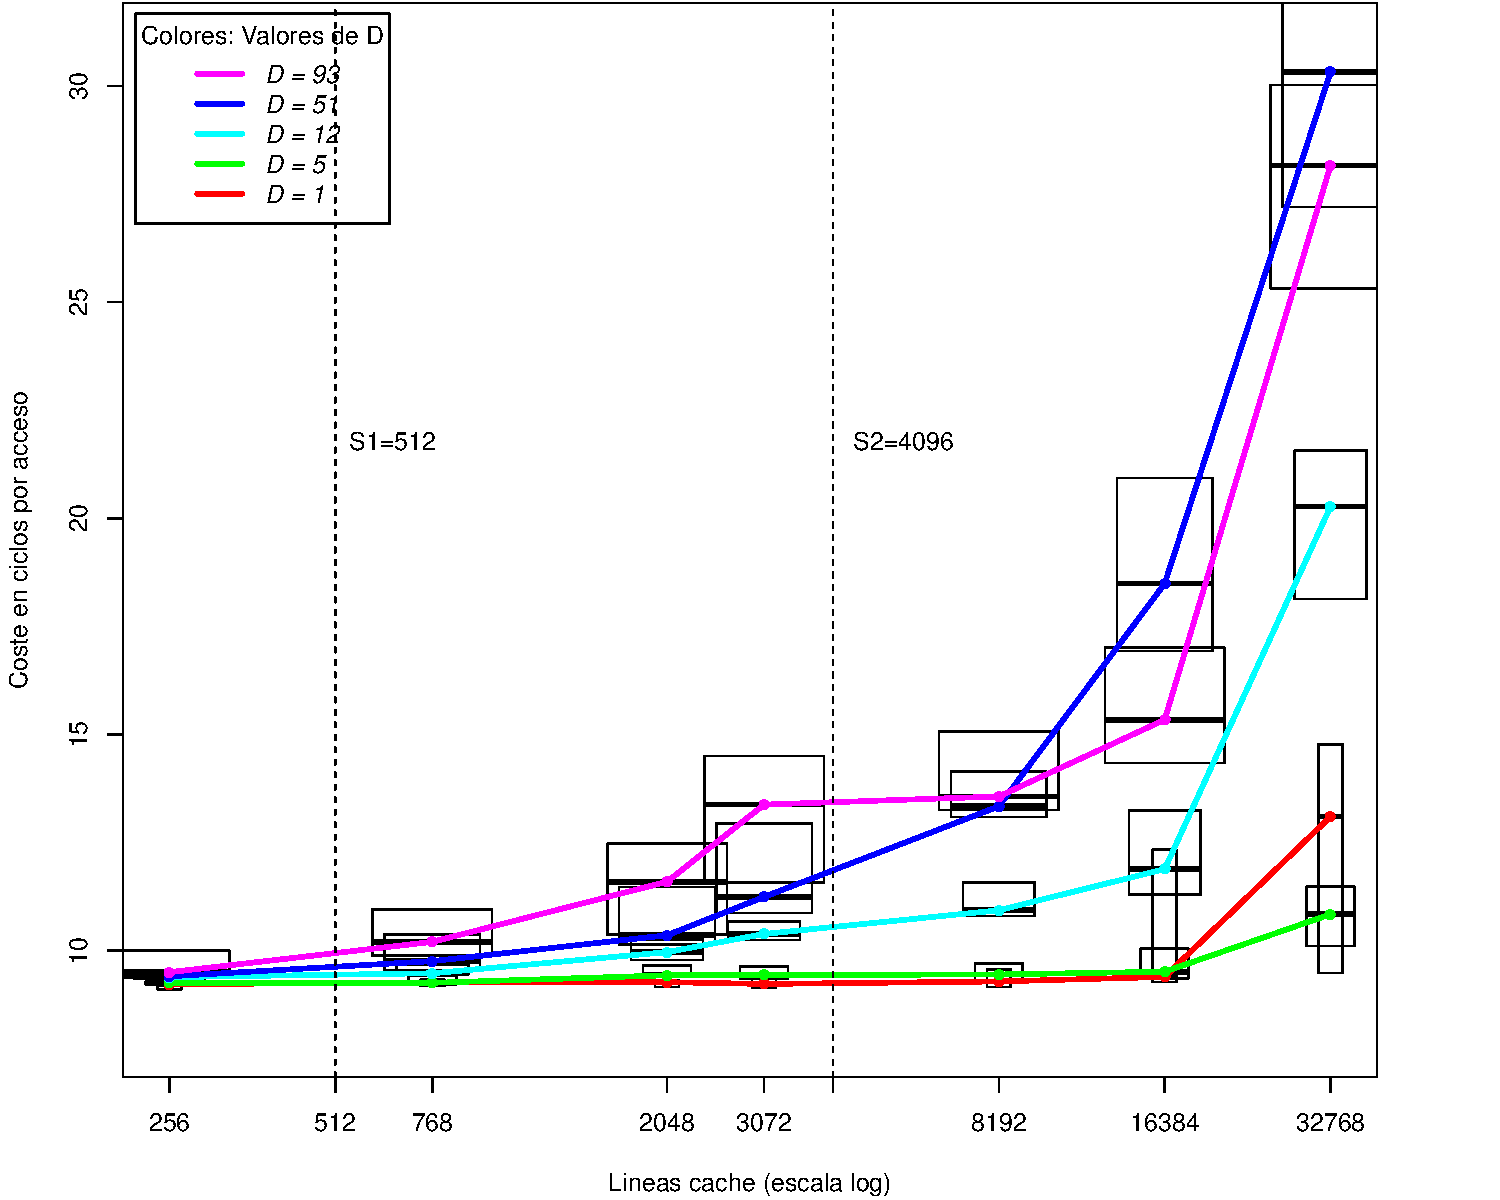
\includegraphics[scale=0.6]{theFile.pdf}
    \caption{Gráfico de resultados}
    \label{fig:g1}
\end{figure*}

\begin{figure*}
  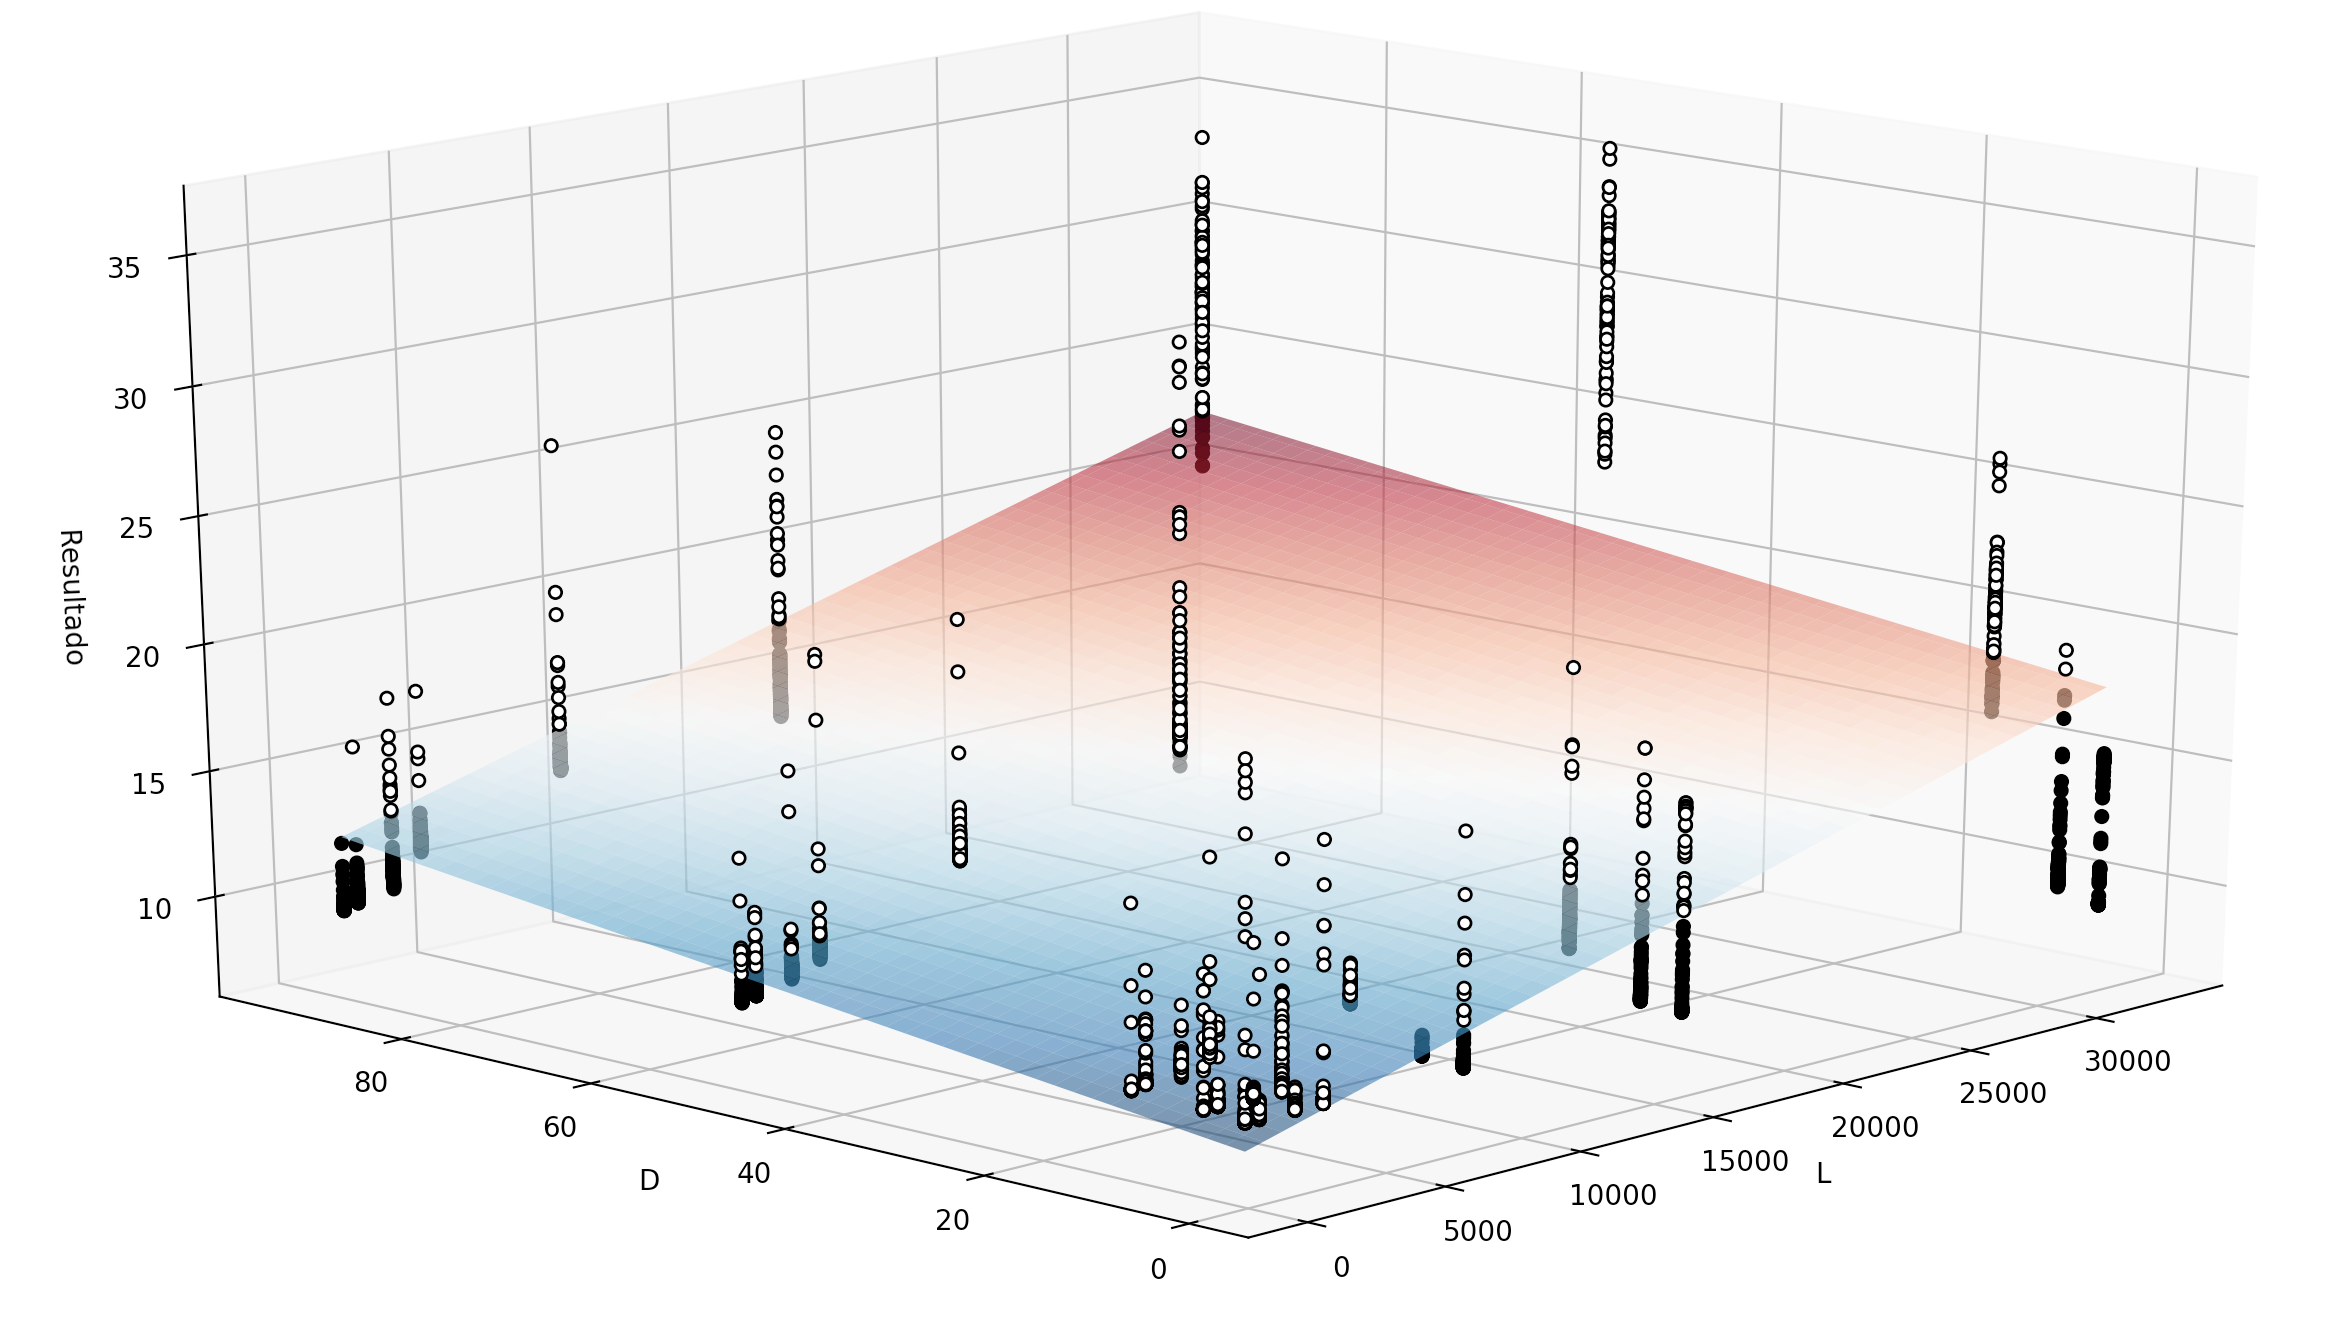
\includegraphics[scale=0.4]{mvRegression.png}
  \centering
  \caption{Regresión multivariante}
  \label{fig:reg}
\end{figure*}

\begin{figure}
  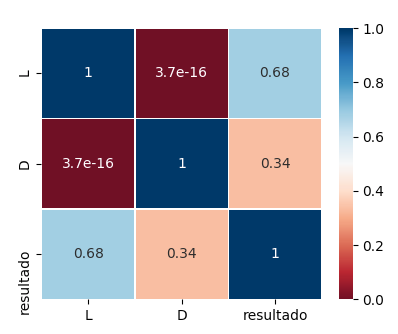
\includegraphics[width=0.7\linewidth]{corr3_3.png}
  \centering
  \caption{Correlación entre os distintos parámetros}
  \label{fig:corr}
\end{figure}
Este feito é aproveitado polo prefetching do procesador. Na arquitectura x86 de Intel, o prefetching só se produce dentro das páxinas de 4KB almacenadas na memoria. Polo tanto estará limitado a unhas 64 liñas caché por diante do dato. Cando se accede secuencialemente a varias direccións próximas, como é o caso para D=1 e D=5, este mecanismo permite reducir notablemente os tempos de carga ao precargar as seguintes direccións antes de que a CPU as pida, e seguramente sexa responsable de manter o custe en ciclos baixos para Ds baixos pese ao aumento de L. 

Por outra banda, a localidade temporal ao repetir a execución dentro do programa fai que para todos os Ds, se L é suficintemente baixo, as respectivas cachés L1, L2 e L3 garden todas as liñas ás que se accedeu recentemente e non faga falta ir aos niveis superiores. Podemos ver claramente como para L = 256 ou 768, o tempo é baixo e seguramente a caché L1 sexa quen de xestionar a maior parte dos accesos a memoria. Polo orde das cifras de acceso, semella que para L = 2048, 3072 e mesmo 8192, a L2 xoga un papel determinante sobre o rendemento e que para Ls máis altos, sobrepasase a súa capacidade.

Isto coincide perfectamente coas marcas na gráfica correpondentes ao tamaño en liñas de L1 e L2, (S1 e S2), polo que temos motivos máis que evidentes para pensar que a capacidade dos distintos niveis de caché marcan o custe en ciclos do acceso a memoria, e segundo se vai sobrepasando a capacidade dos distintos niveis de cache, suben os ciclos de forma acorde ao rendemento característico con ese nivel da caché.

Para confirmar este comportamento, estudamos os fallos e accesos aos distintos niveis de caché mediante a librería PAPI que le contadores hardware do procesador. Sería bastante máis doado usando a interface perf do kernel linux, que permite acceder a estes contadores directamente dende a consola, pero ao non dispoñer de acceso como superusuario no entorno de execución, non era posible utilizar esta ferramenta nin obter a librería PAPI automaticamente usando un xestor de paquetes.

Tamén tivemos dificultades debido á naturaleza do i3-3240 do entorno de execución: ten moi poucos contadores hardware dispoñibles, e en certas combinacións deixan de funcionar. Ademáis, certos parámetros como o número de accesos a L1 non son medibles neste procesador, polo que ó final tivemos que conformarnos coas seguintes métricas: fallos caché de L1, L2 e L3, accesos caché totales de L2 e L3, e total de instruccións SW e LW durante a execución.

\begin{figure}
    \centering
    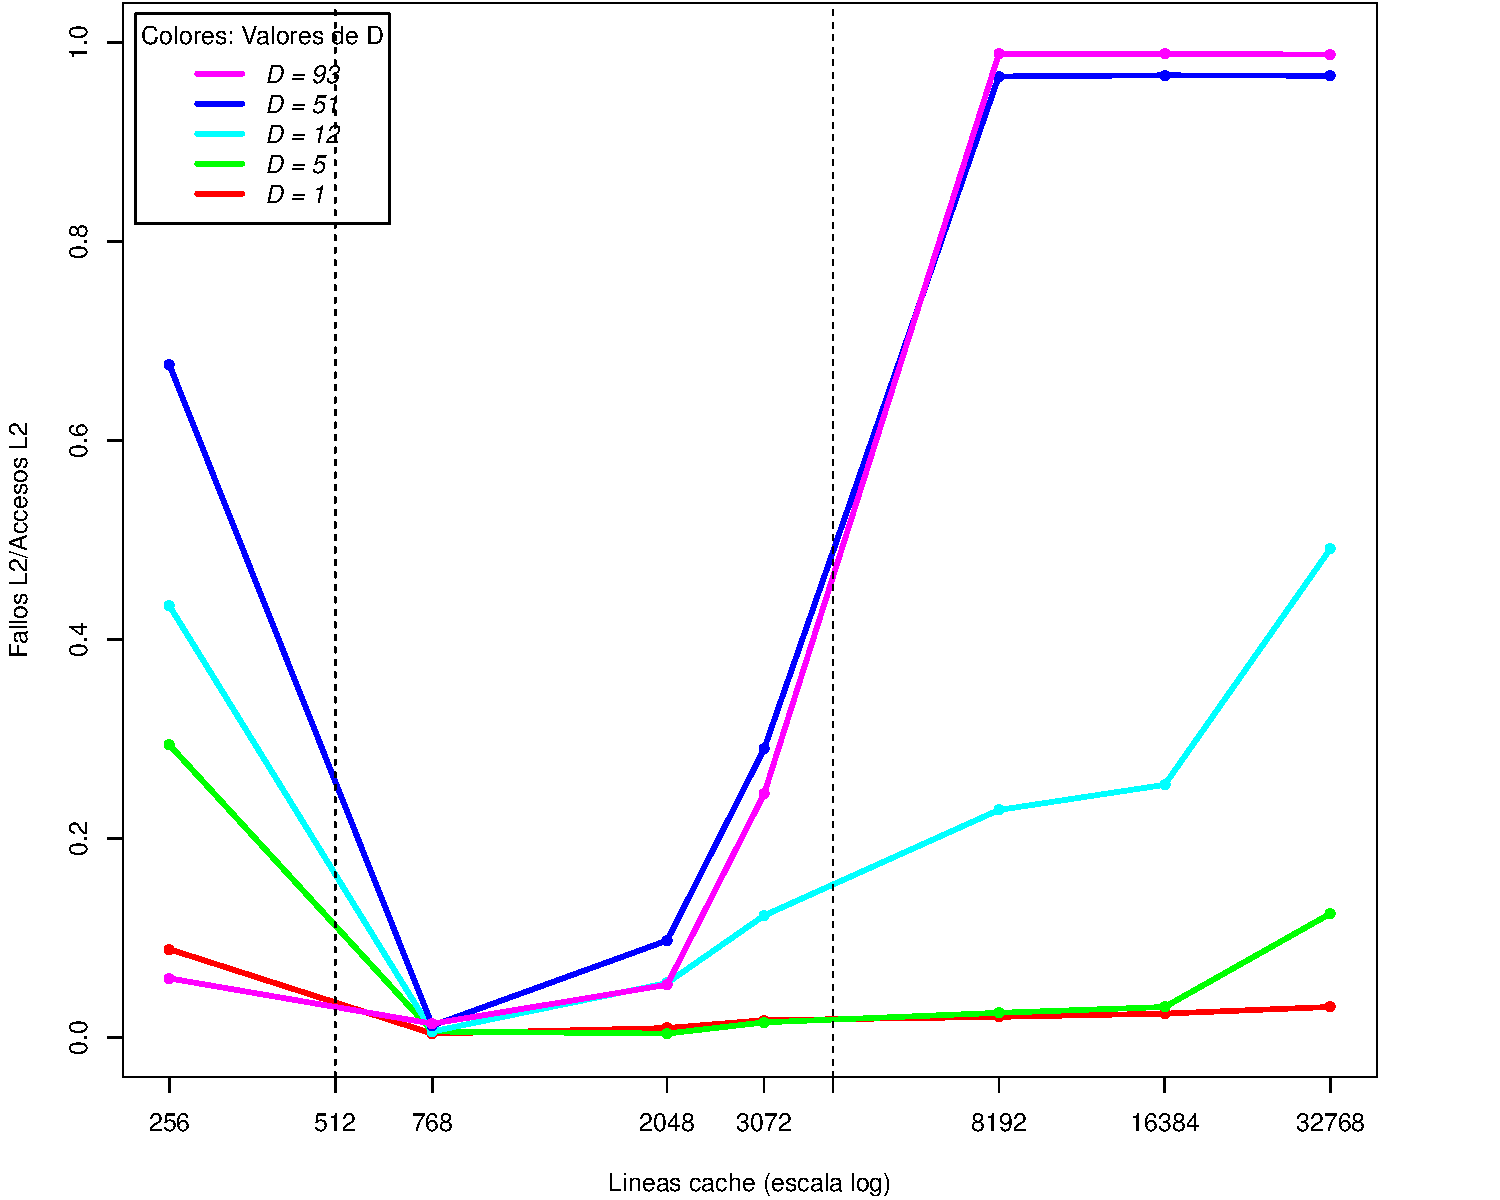
\includegraphics[scale=0.38]{L2M-L2A.pdf}
    \caption{Taxa de fallos de L2}
    \label{fig:papil2}
\end{figure}

O resultado confirma totalmente as hipóteses: na figura \ref{fig:papil2} (taxa de fallos de L2) vese cómo xustamente para os Ls da súa capacidade, descende radicalmente a taxa de fallos a 0, e cando L sobrepasa a súa capacidade, a taxa de fallos para Ds grandes tende a 1. Resulta ilóxico que para L=256 aparezan bastante fallos, pero isto, tal e como se na figura \ref{fig:papil2t}(fallos cache/(instruccións SW + instruccións LW)), é despreciable pola puoca cantidade de accesos que fai a L2 para L=256.  


\begin{figure}
    \centering
    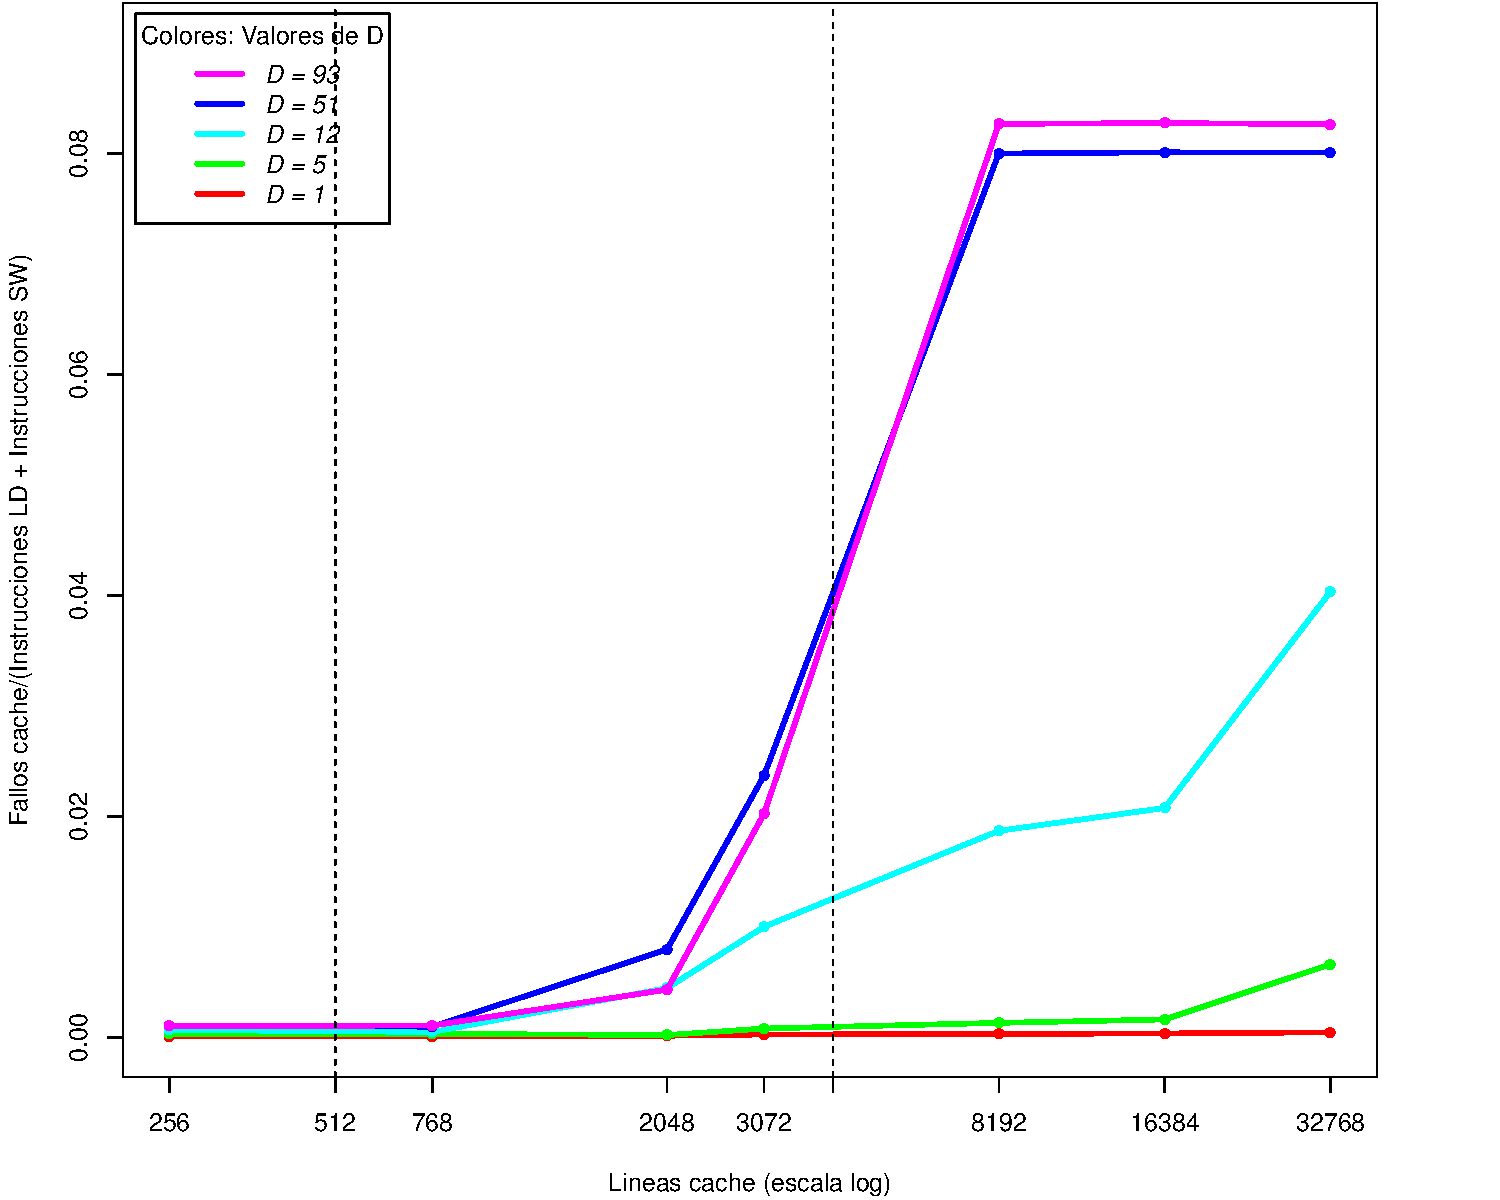
\includegraphics[scale=0.38]{L2M-T.pdf}
    \caption{Fallos L2/(instruccións SW + instruccións LW)}
    \label{fig:papil2t}
\end{figure}

Se nos fixamos nos fallos de L3 / instruccións (figura \ref{fig:papil3}, a taxa de fallos da caché como tal é pouco representativa por ser poucos os accesos que chegan ata L3 para algunhas combinacións de L e D), vemos como se mantén relativamente baixa en todos os valores e só repunta lixeiramente para L e Ds altos. De novo, todo segundo o esperado nas hipóteses.

\begin{figure}
    \centering
    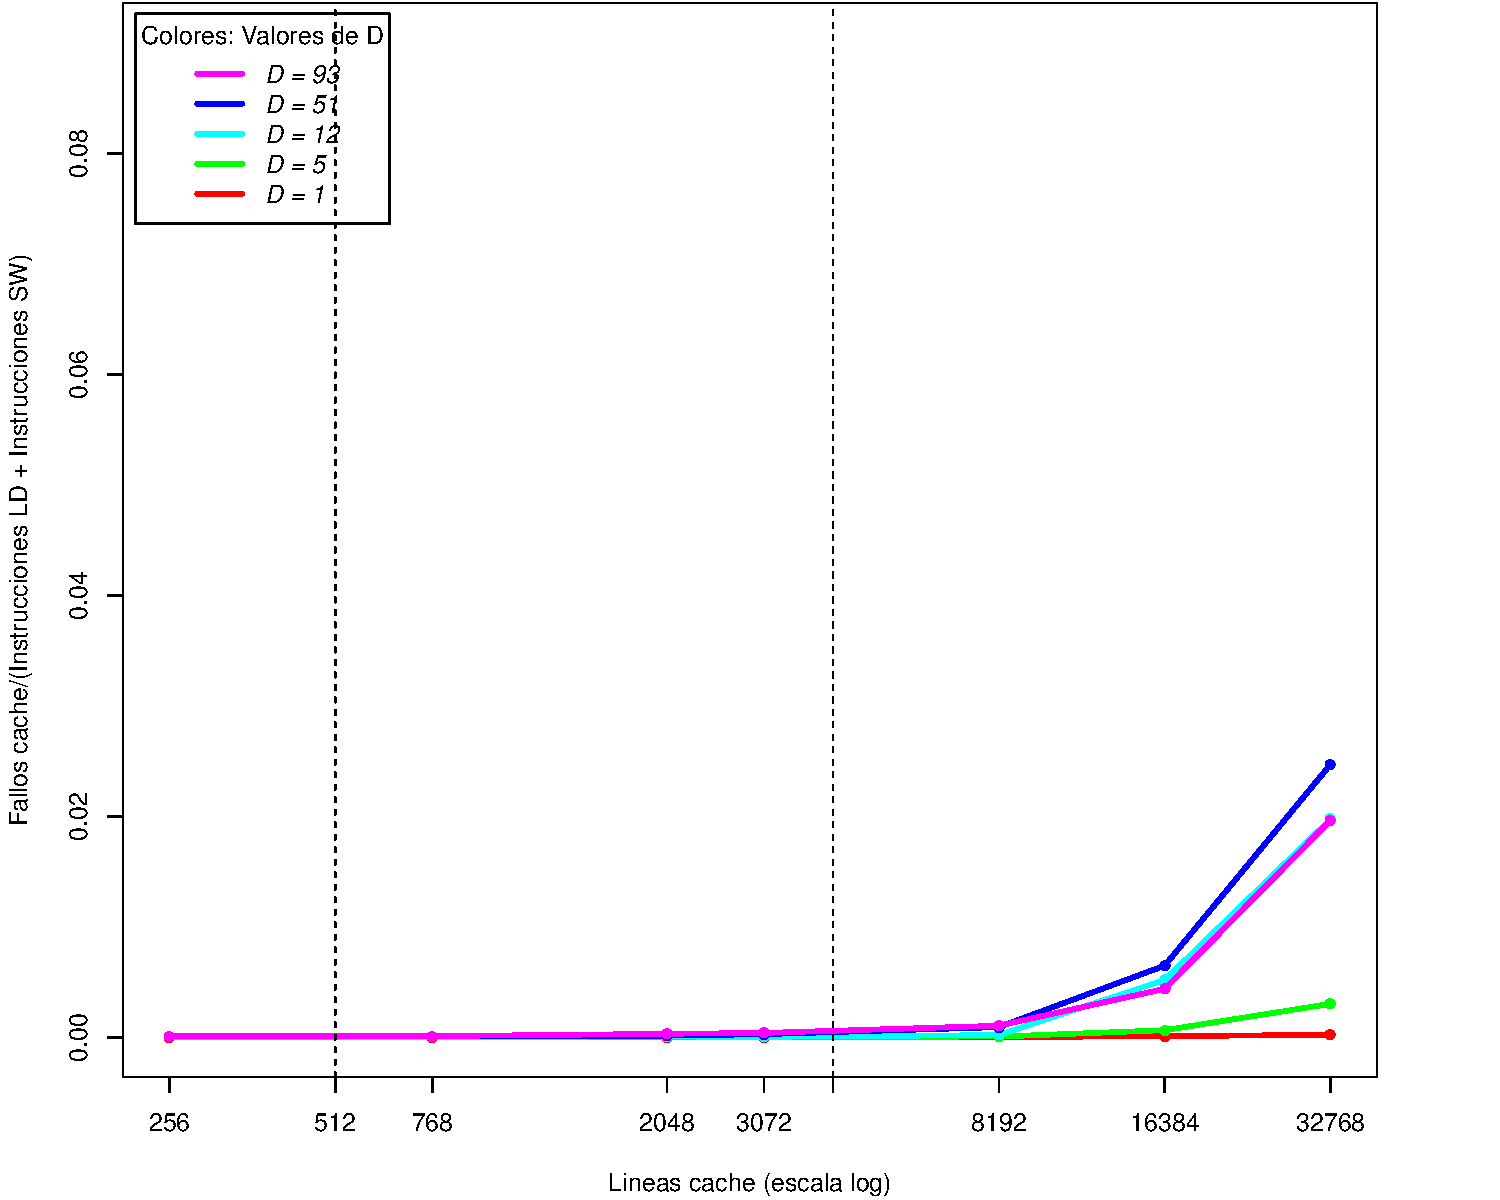
\includegraphics[scale=0.38]{L3M-T.pdf}
    \caption{Fallos L3/(instruccións SW + instruccións LW)}
    \label{fig:papil3}
\end{figure}

Por último, para L1 non podemos calcular a taxa de fallos por non dispoñer dos accesos totales. Sen embargo, si podemos comparar os fallos de L1 cos de L2 e tamén podemos comparalos cos accesos totales. Na figura \ref{fig:papil1t} o comportamento é o esperado: os fallos son baixos para L=256 e suben a partir dese punto por sobrepasarse a capacidade de L1. Comparando os fallos de L1 cos de L2 (figura \ref{fig:papil1l2}), observamos como ambas fallan por igual para Ls grandes, falla moito máis L1 que L2 entre S1 e S2 e falla menos L1 para L=256.

\begin{figure}
    \centering
    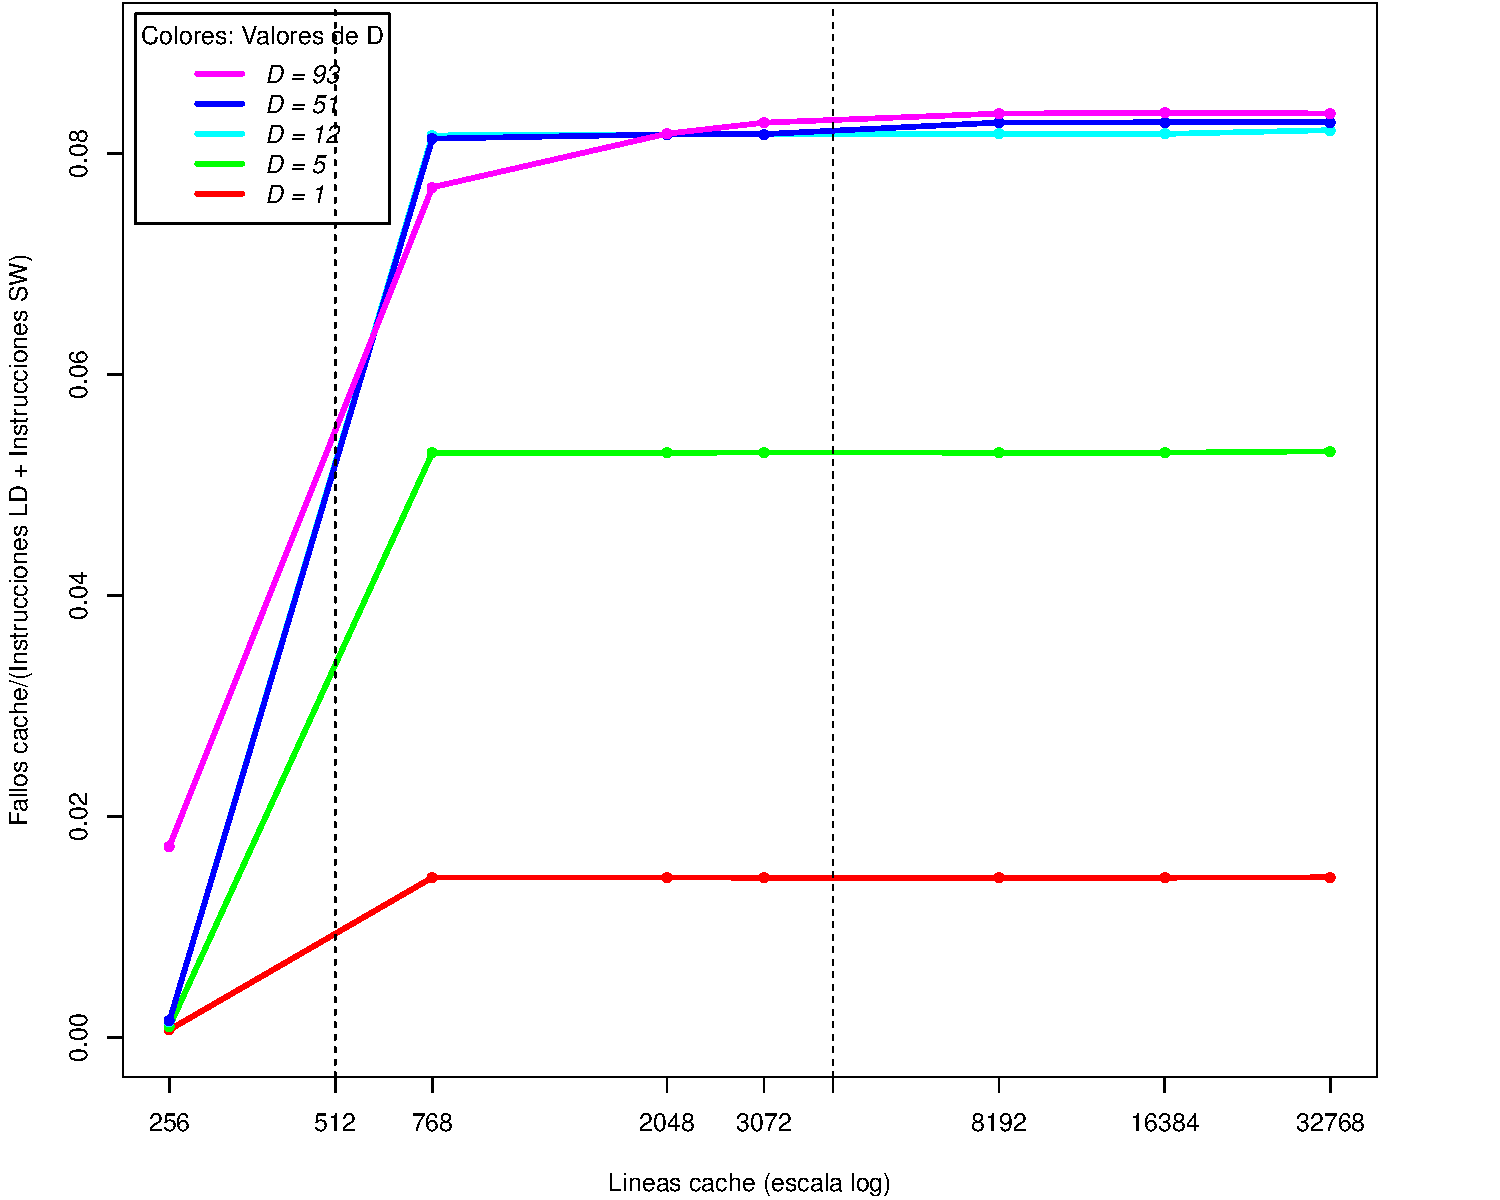
\includegraphics[scale=0.38]{L1M-T.pdf}
    \caption{Fallos L1/(instruccións SW + instruccións LW)}
    \label{fig:papil1t}
\end{figure}

\begin{figure}
    \centering
    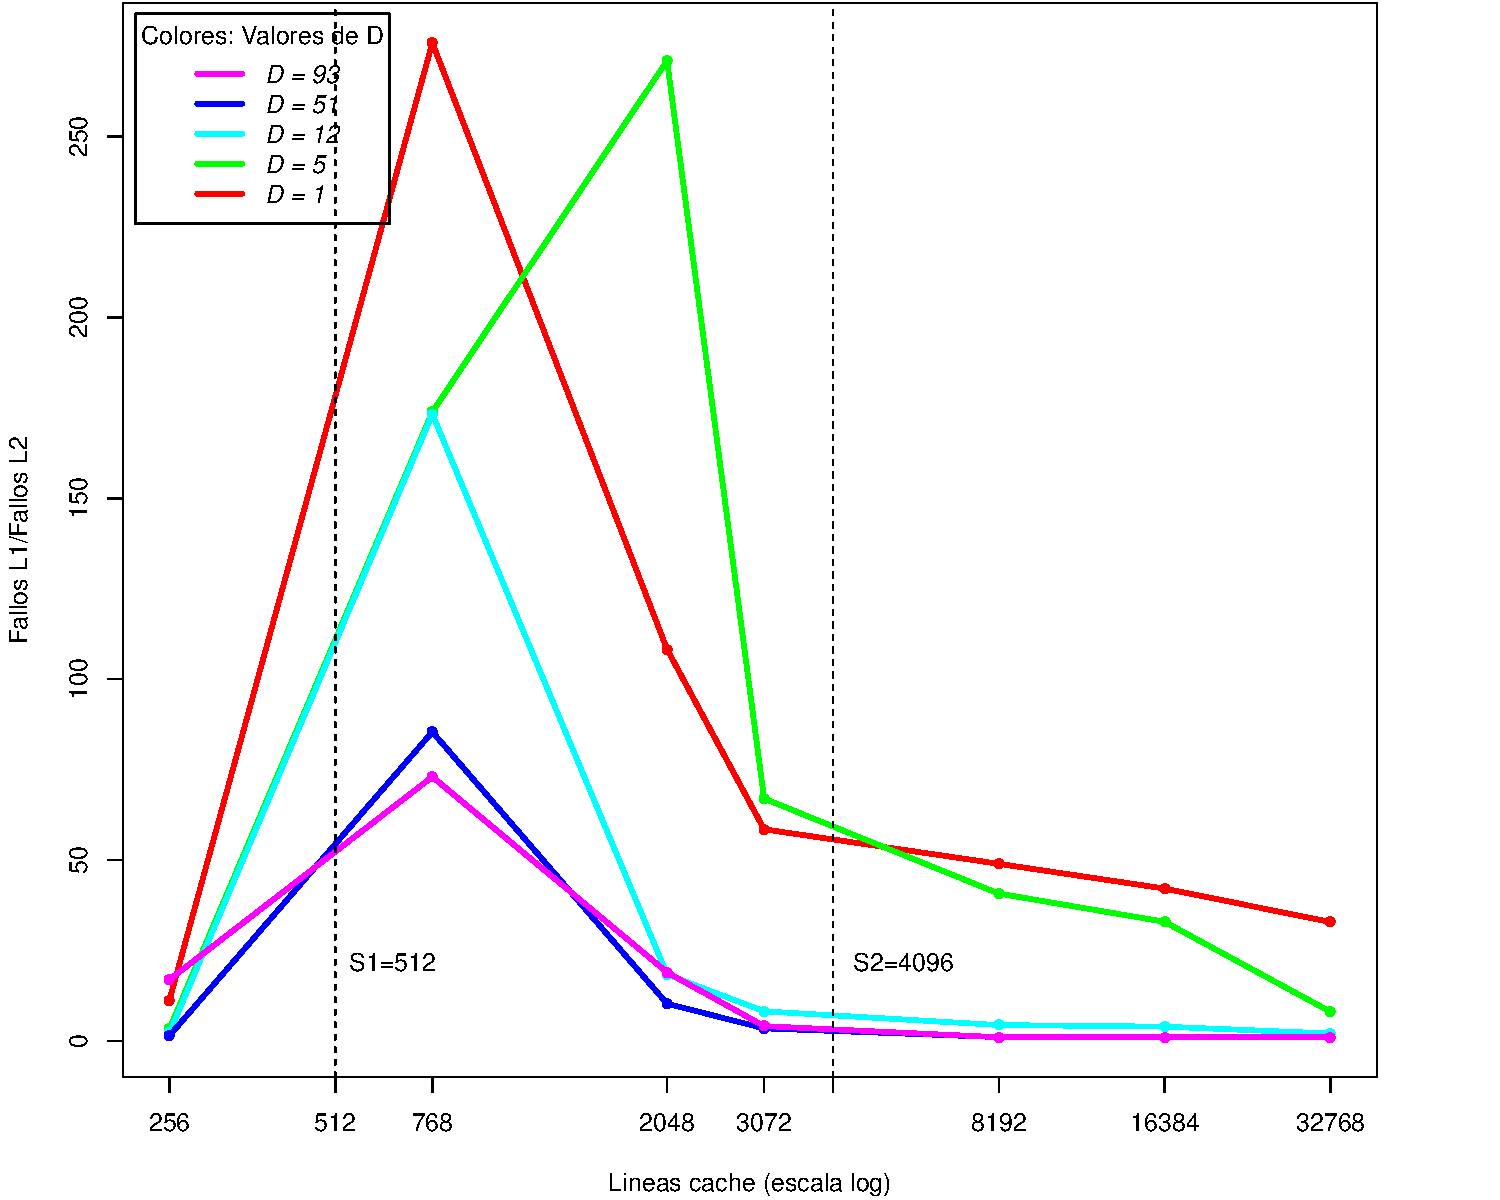
\includegraphics[scale=0.38]{L1M-L2M.pdf}
    \caption{Fallos L1/Fallos L2}
    \label{fig:papil1l2}
\end{figure}


\section{Conclusións}

Como vimos ao longo deste documento, o principio de localidade e o prefetching xogan un papel crucial no rendemento dun código, polo que é interesante tratar de exprimir ambas características á hora de construir programas eficientes. En xeral, trataremos de que o patrón de acceso aos datos sexa regular e fomentaremos o uso dos mesmos datos de forma concentrada e repetida no código.

Nos últimos anos, o desenvolvemento da tecnoloxía acadou un punto no cal a meirande parte das estratexias que melloran a localidade ou o prefetching son incorporadas ao noso programa de xeito automático, ben polos compiladores ou ben polo propio hardware. Por unha parte, os procesadores actuais contan cun mecanismo que permite realizar o prefetching a nivel de hardware. Por outra banda, os compiladores, como é o caso do gcc, contan con diversos mecanismos automticos e flags que permiten mellorar a localidade do código.

Non obstante, a pesar de todos estes avances, aínda queda un longo percorrido ata conseguir que todas as optimizacións sexan realizadas sen necesidade de intervención humana. Linguaxes de programación como C, permiten ao programador controlar aspectos como o prefetching mediante a instrucións específicas. Este prefetching a nivel de software só resulta útil cando existe un acceso regular ao array de cuxos elementos se fixo prefetching, xa que o programador debe determinar de xeito explícito no código a que elementos se debe de facer o prefetch. Pola contra, o prefetching de hardware funciona de xeito dinámico, baseado no comportamento do programa en tempo de execución. Do mismo modo, as técnicas que permiten mellorar o efecto do principio de localidade son numerosas, entre as cales destacan algunhas blocking ou loop interchange. En todo caso, sempre é conveniente ter en conta a construcción do hardware de cara a programación, posto que isto pode variar considerablemente a elección da estratexia de optimización.

En resumo, a pesar de que a área de optimización dentro da arquitectura de computadores sexa moi amplia, ao longo deste documento foi posible observar como tanto o prefetching coma o principio de localidade son aspectos que deben ser tidos en conta á hora de deseñar programas, posto que un bo uso destes dous conceptos pode ter consecuencias drásticas no tempo de execución dun programa.

%%%%%%%%%%%%%%%%%%%%%%%%%%%%%%%%%%%%%%%%%%%%%%%%%%%%%%%%%%%%%%%%%%%%%%%%%%%%%%%%

%%%%%%%%%%%%%%%%%%%%%%%%%%%%%%%%%%%%%%%%%%%%%%%%%%%%%%%%%%%%%%%%%%%%%%%%%%%%%%%%


\begin{thebibliography}{99}

\bibitem{c1} CPU-World. Intel Core i3-3240 specifications. \url{http://www.cpu-world.com/CPUs/Core_i3/Intel-Core\%20i3-3240.html}







\end{thebibliography}




\end{document}
